\documentclass[12pt,openany,oneside,a4paper,chapter=TITLE,english,brazil]{abntex2}

\usepackage{fontspec}
\setmainfont{texgyretermes}[Extension=.otf,UprightFont=*-regular,BoldFont=*-bold,ItalicFont=*-italic,BoldItalicFont=*-bolditalic]
\setmonofont{DejaVuSansMono}[Extension=.ttf,Scale=0.82,BoldFont=*-Bold,ItalicFont=*-Oblique,BoldItalicFont=*-BoldOblique]
\usepackage{newunicodechar}
\newunicodechar{↔}{\ensuremath{\leftrightarrow}}
\newunicodechar{∥}{\ensuremath{\parallel}}
\usepackage{xcolor}
\usepackage{graphicx}
\graphicspath{{../}}
\usepackage{tabularx,array,booktabs}
\usepackage{placeins}
\usepackage{fvextra}
\RecustomVerbatimEnvironment{verbatim}{Verbatim}{breaklines,breakanywhere,fontsize=\footnotesize,frame=single,framesep=2mm}
\usepackage{mdframed}
\usepackage{xurl}
\urlstyle{same}
\usepackage{microtype}

\renewcommand{\ABNTEXchapterfont}{\rmfamily\bfseries\raggedright\hyphenpenalty=10000\exhyphenpenalty=10000}
\renewcommand{\ABNTEXsectionfont}{\rmfamily\bfseries\raggedright\hyphenpenalty=10000\exhyphenpenalty=10000}
\renewcommand{\ABNTEXsubsectionfont}{\rmfamily}
\renewcommand{\ABNTEXsubsubsectionfont}{\rmfamily\itshape}
\makeatletter
\renewcommand{\ABNTEXchapterupperifneeded}[1]{%
  \ifthenelse{\boolean{abntex@innonumchapter}\OR\boolean{abntex@apendiceousecao}}{}{\raggedright}%
  \ifthenelse{\boolean{ABNTEXupperchapter}}{\MakeTextUppercase{#1}}{#1}}
\makeatother
\providecommand{\tightlist}{\setlength{\itemsep}{0pt}\setlength{\parskip}{0pt}}
\providecommand{\pandocbounded}[1]{#1}

\newcommand{\quadroname}{Quadro}
\newcommand{\listofquadrosname}{Lista de quadros}
\newfloat[chapter]{quadro}{loq}{\quadroname}
\newlistof{listofquadros}{loq}{\listofquadrosname}
\newlistentry{quadro}{loq}{0}
\setfloatadjustment{quadro}{\centering}
\counterwithout{quadro}{chapter}
\renewcommand{\cftquadroname}{\quadroname\space}
\renewcommand*{\cftquadroaftersnum}{\hfill--\hfill}
\setfloatlocations{quadro}{!htbp}

\renewcommand{\topfraction}{0.9}
\renewcommand{\bottomfraction}{0.8}
\renewcommand{\textfraction}{0.07}
\renewcommand{\floatpagefraction}{0.8}
\setcounter{topnumber}{3}
\setcounter{bottomnumber}{2}
\setcounter{totalnumber}{4}
\makeatletter
\setlength{\@fptop}{0pt}
\setlength{\@fpsep}{12pt}
\setlength{\@fpbot}{0pt plus 1fil}
\makeatother

\newenvironment{referenciasabnt}
  {\begin{flushleft}\SingleSpacing\setlength{\parindent}{0pt}\setlength{\parskip}{\baselineskip}}
  {\end{flushleft}}

\titulo{eBPF e Cilium sem mistério: do primeiro hook à carga do programa}
\autor{Learn Cilium}
\local{Teresina}
\data{2026}
\preambulo{Edição 0.1 piloto. Público-alvo: iniciantes.}

\makeatletter
\hypersetup{
  pdftitle={\@title},
  pdfauthor={\@author},
  pdfsubject={Laboratório Kubernetes, Cilium e BGP},
  pdfkeywords={Cilium}{BGP}{Gateway API}{Kubernetes}{eBPF},
  colorlinks=true,
  linkcolor=black,
  citecolor=black,
  urlcolor=blue!50!black,
  bookmarksdepth=4
}
\makeatother

\setlrmarginsandblock{3cm}{2cm}{*}
\setulmarginsandblock{3cm}{2cm}{*}
\checkandfixthelayout
\setlength{\parindent}{1.3cm}
\setlength{\parskip}{0.2cm}
\setlength{\emergencystretch}{5em}
\tolerance=1000

\begin{document}
\selectlanguage{brazil}
\renewcommand{\listfigurename}{Lista de figuras}
\frenchspacing

\imprimircapa
\imprimirfolhaderosto

\pretextualchapter{Apresentação}
Este piloto acompanha um programa eBPF --- um programa restrito que o kernel Linux pode carregar --- do pedido de carga até um evento. O kernel é o núcleo do Linux; hook é um ponto previsto de ligação, e evento é a ocorrência que chega àquele contexto. Espaço de usuário é a área fora do kernel onde processos executam; ali, o agente do Cilium configura componentes, enquanto o programa ligado ao hook atua no contexto do kernel. O caminho exato depende do tipo de programa e da configuração.

Vocabulário de configuração: YAML é um formato textual para dados. No Kubernetes, label (rótulo) é um par chave/valor de metadados que ajuda a identificar e selecionar objetos, mas não autentica; no exemplo ilustrativo \texttt{app:\allowbreak{} api}, \texttt{app} é a chave e \texttt{api} é o valor (Kubernetes Authors, 2026). Um manifesto Kubernetes é um documento declarativo que descreve um recurso; policy (política de tráfego) é uma regra declarada para controlar comunicações (Cilium Authors, 2026). Nas citações autor-data, 2026 é o ano de consulta quando a página não informa o ano de publicação; \texttt{[s.\allowbreak{}d.\allowbreak{}]} nas referências conserva essa ausência sem inventar data.

As figuras são modelos didáticos originais. O fragmento YAML e os nomes \texttt{frontend}, \texttt{api} e \texttt{backend} são exemplos ilustrativos; não descrevem um cluster observado. A documentação stable do Cilium consultada em 28 de outubro de 2026 indicava 1.20.4; isso é referência documental, não versão instalada ou executada.


\pdfbookmark[0]{\listfigurename}{lof}
\listoffigures*
\cleardoublepage
\pdfbookmark[0]{\listofquadrosname}{loq}
\listofquadros*
\cleardoublepage
\pdfbookmark[0]{\listtablename}{lot}
\listoftables*
\cleardoublepage
\pdfbookmark[0]{\contentsname}{toc}
\tableofcontents*
\cleardoublepage

\textual
\OnehalfSpacing

\chapter{Um programa eBPF encontra seu evento}\label{um-programa-ebpf-encontra-seu-evento}

\section{O que você vai aprender}\label{o-que-vocuxea-vai-aprender}

Ao final, você poderá:

\begin{itemize}
\tightlist
\item
  explicar com palavras simples o que é um hook e onde um programa eBPF se conecta;
\item
  ordenar solicitação de carga, verificação, aceitação ou rejeição, attach e execução por evento;
\item
  distinguir o que a aprovação do verifier indica daquilo que ela não prova, e separar o agente Cilium do datapath.
\end{itemize}

\textbf{Pré-requisito:} nenhum cluster ou terminal. Leia a sequência como um modelo conceitual; ela não é uma receita de instalação.

\section{Palavras antes do jargão}\label{palavras-antes-do-jarguxe3o}

\begin{quadro}[!htbp]
\caption{Vocabulário em uma frase}
\footnotesize
\begin{tabularx}{\textwidth}{|>{\raggedright\arraybackslash\hsize=0.586\hsize}X|>{\raggedright\arraybackslash\hsize=1.414\hsize}X|}
\hline
\textbf{Termo} & \textbf{Definição curta e limite} \\
\hline
Kernel / eBPF & O kernel é o núcleo do Linux; eBPF carrega programas restritos que
respondem a certos eventos. \\
\hline
Hook / evento & Hook é um ponto previsto de ligação; evento é a ocorrência que chega a
esse contexto. \\
\hline
Verifier / mapa & Verifier analisa propriedades de segurança na carga; mapa guarda valores
associados a chaves. \\
\hline
Attach / JIT & Attach liga um programa aceito ao hook; JIT compila para instruções
nativas quando aplicável. \\
\hline
Agente / datapath & O agente Cilium configura componentes; o datapath processa tráfego. Cada
um tem um papel diferente. \\
\hline
\end{tabularx}
\fonte{Elaboração própria (2026), com base em (eBPF Foundation, 2026), (Linux
Kernel Documentation, 2026) e (Cilium Authors, 2026).}
\end{quadro}

\section{Um ponto de ligação, dois papéis}\label{um-ponto-de-ligauxe7uxe3o-dois-papuxe9is}

A analogia do hook como ponto de conexão ajuda a localizar o attach; ele não é um guarda geral, e contexto e resultado variam por tipo.

\begin{figure}[!htbp]
\caption{O agente configura; o programa atua no hook}
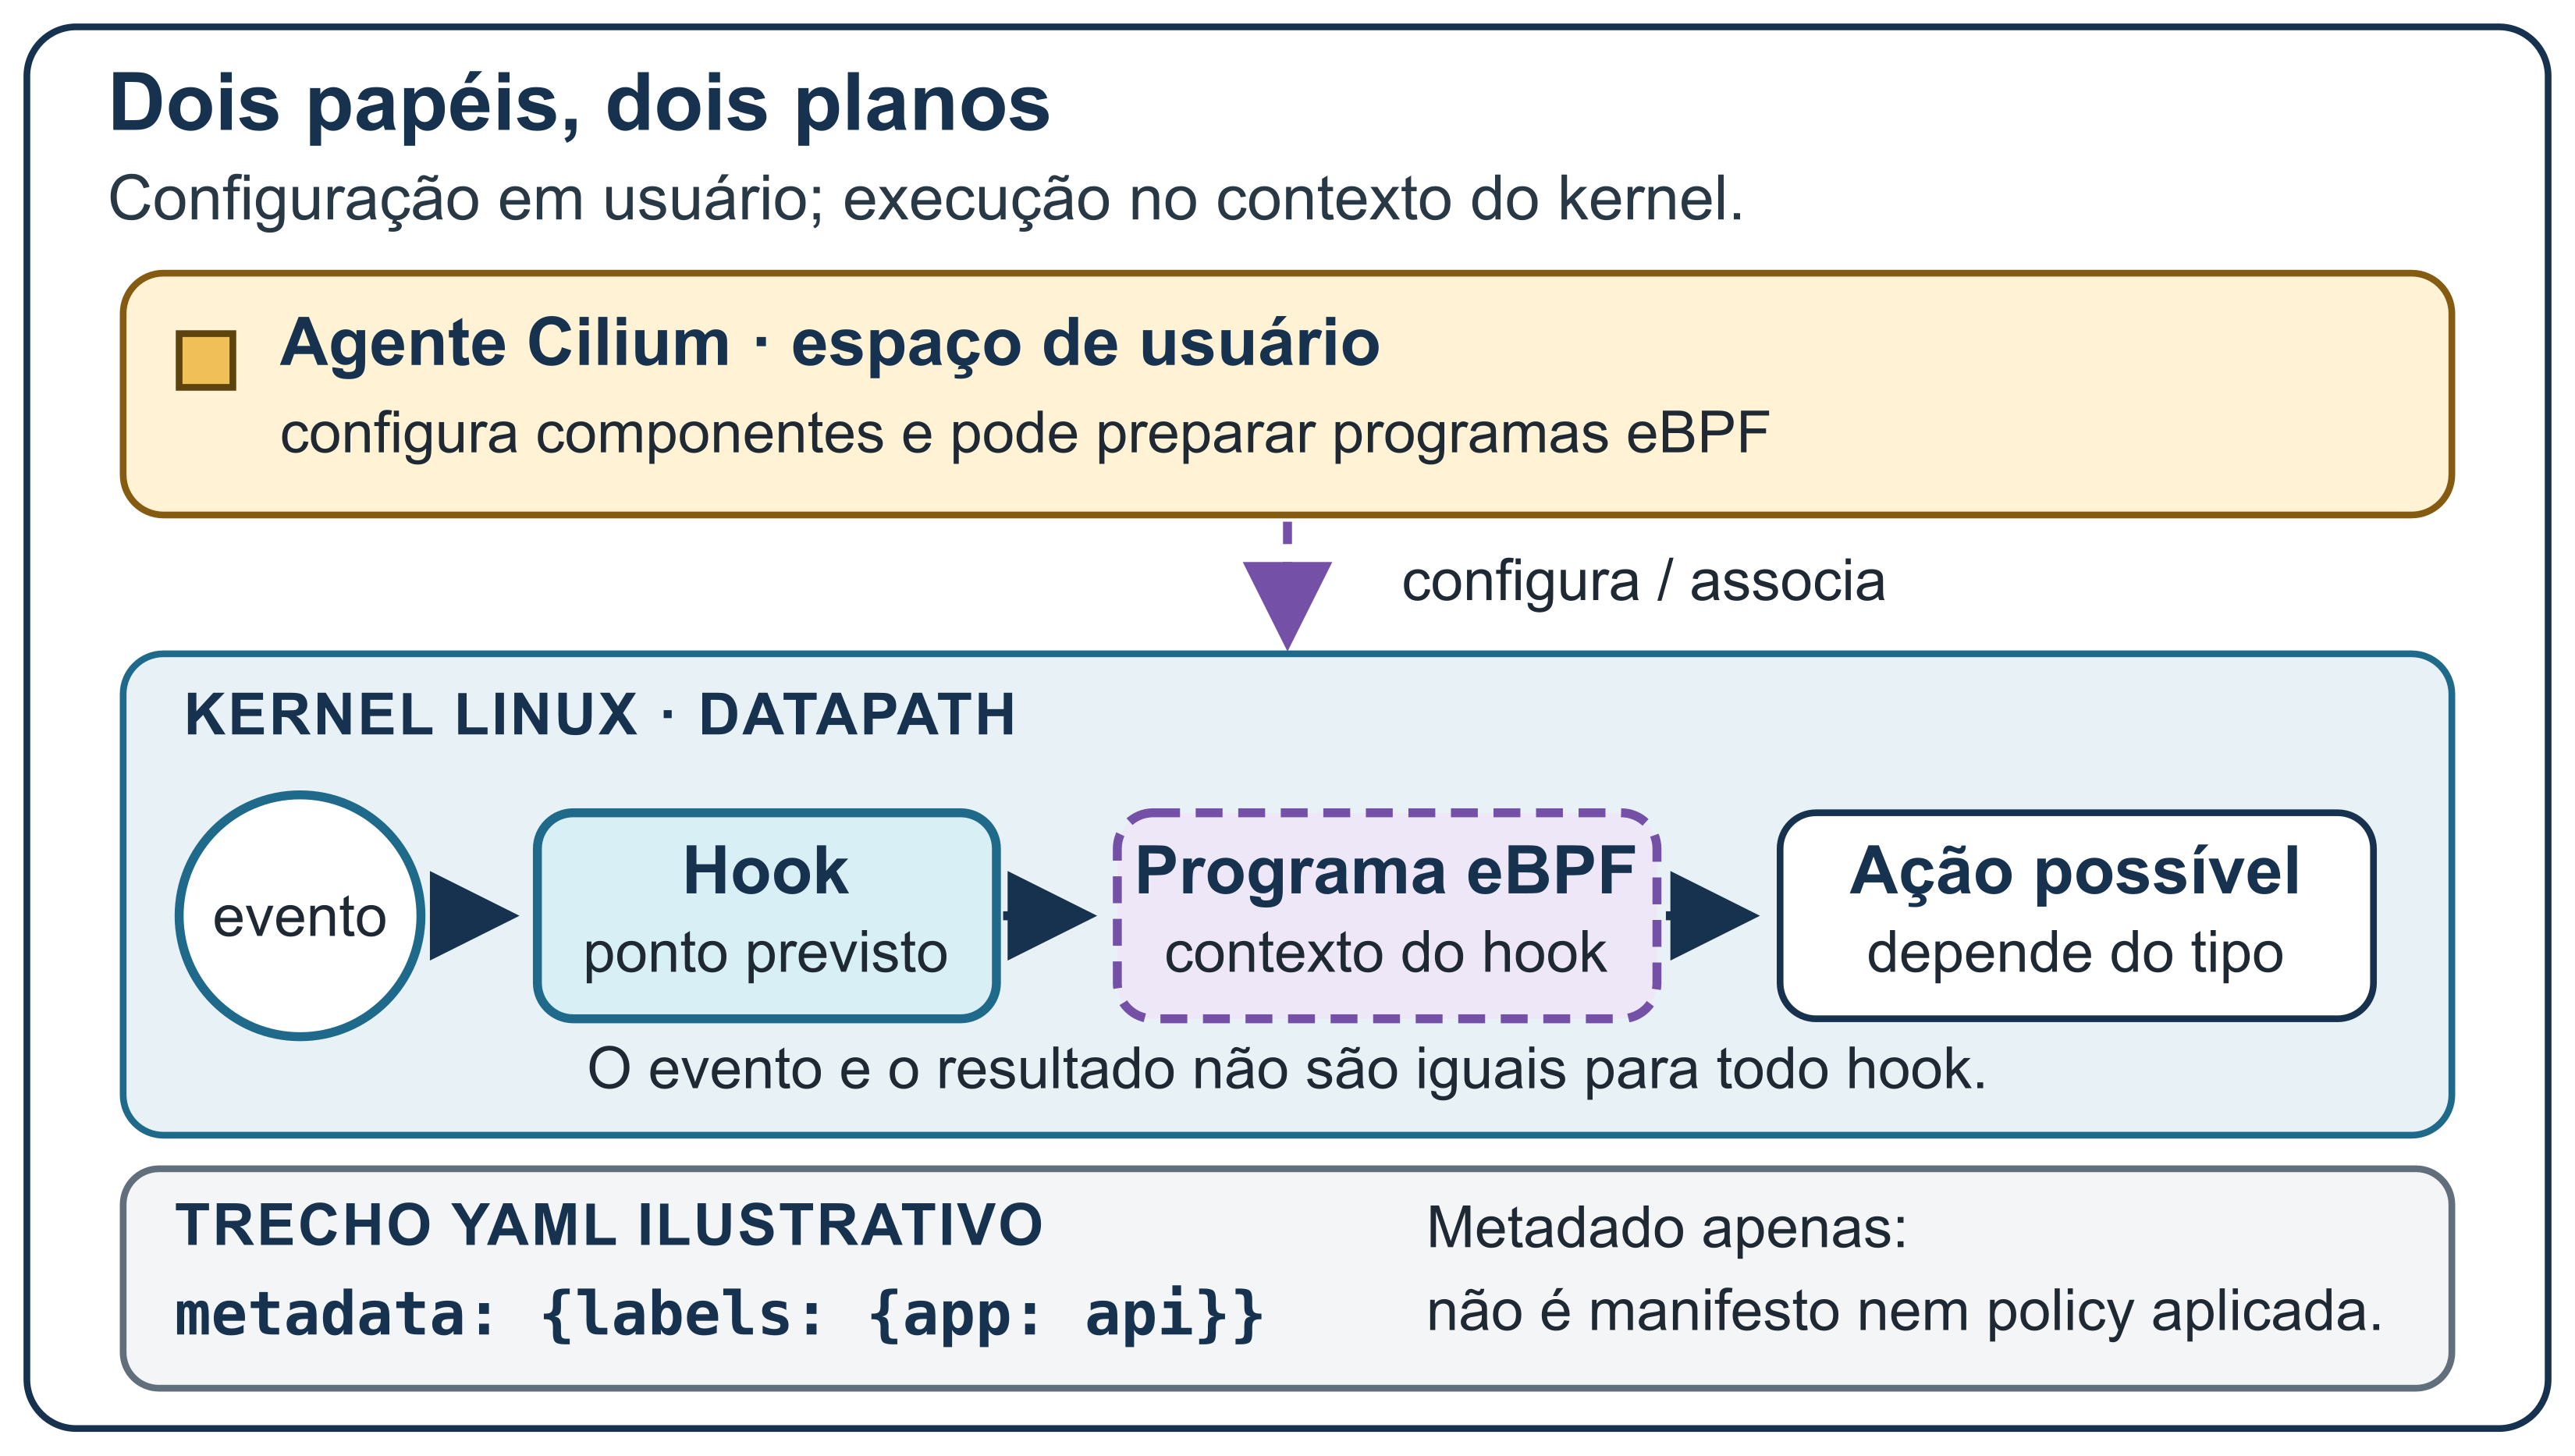
\includegraphics[width=\textwidth,height=0.72\textheight,keepaspectratio]{diagramas/ebpf-cilium-iniciantes/figura-01-papeis.png}
\fonte{Elaboração própria (2026), com base em (Cilium Authors, 2026), (eBPF
Foundation, 2026) e (Kubernetes Authors, 2026).}
\end{figure}

Leitura da Figura 1: agente configura; no kernel, evento → hook → programa → ação por tipo. O fragmento YAML \texttt{metadata:\allowbreak{} \{labels:\allowbreak{} \{app:\allowbreak{} api\}\}} é ilustrativo, não manifesto nem policy aplicada; label não autentica. (Kubernetes Authors, 2026).

\section{Da solicitação ao evento}\label{da-solicitauxe7uxe3o-ao-evento}

No modelo temporal, um loader em espaço de usuário solicita a carga ao kernel. O verifier do kernel analisa o programa; se rejeita, a tentativa termina. Se aceita, o kernel pode compilar com JIT quando aplicável. Então o loader solicita attach, o kernel associa o programa ao hook e um evento compatível chega ao hook, onde o programa executa no contexto do kernel. Esta é uma sequência didática, pois os mecanismos de carga e attach variam por tipo de programa. (eBPF Foundation, 2026; Linux Kernel Documentation, 2026; Cilium Authors, 2026)

No caminho rejeitado, a tentativa termina; no caminho aceito, JIT permanece condicional e o loader pede attach ao kernel.

\begin{figure}[!htbp]
\caption{Sequência temporal: loader, kernel e hook}
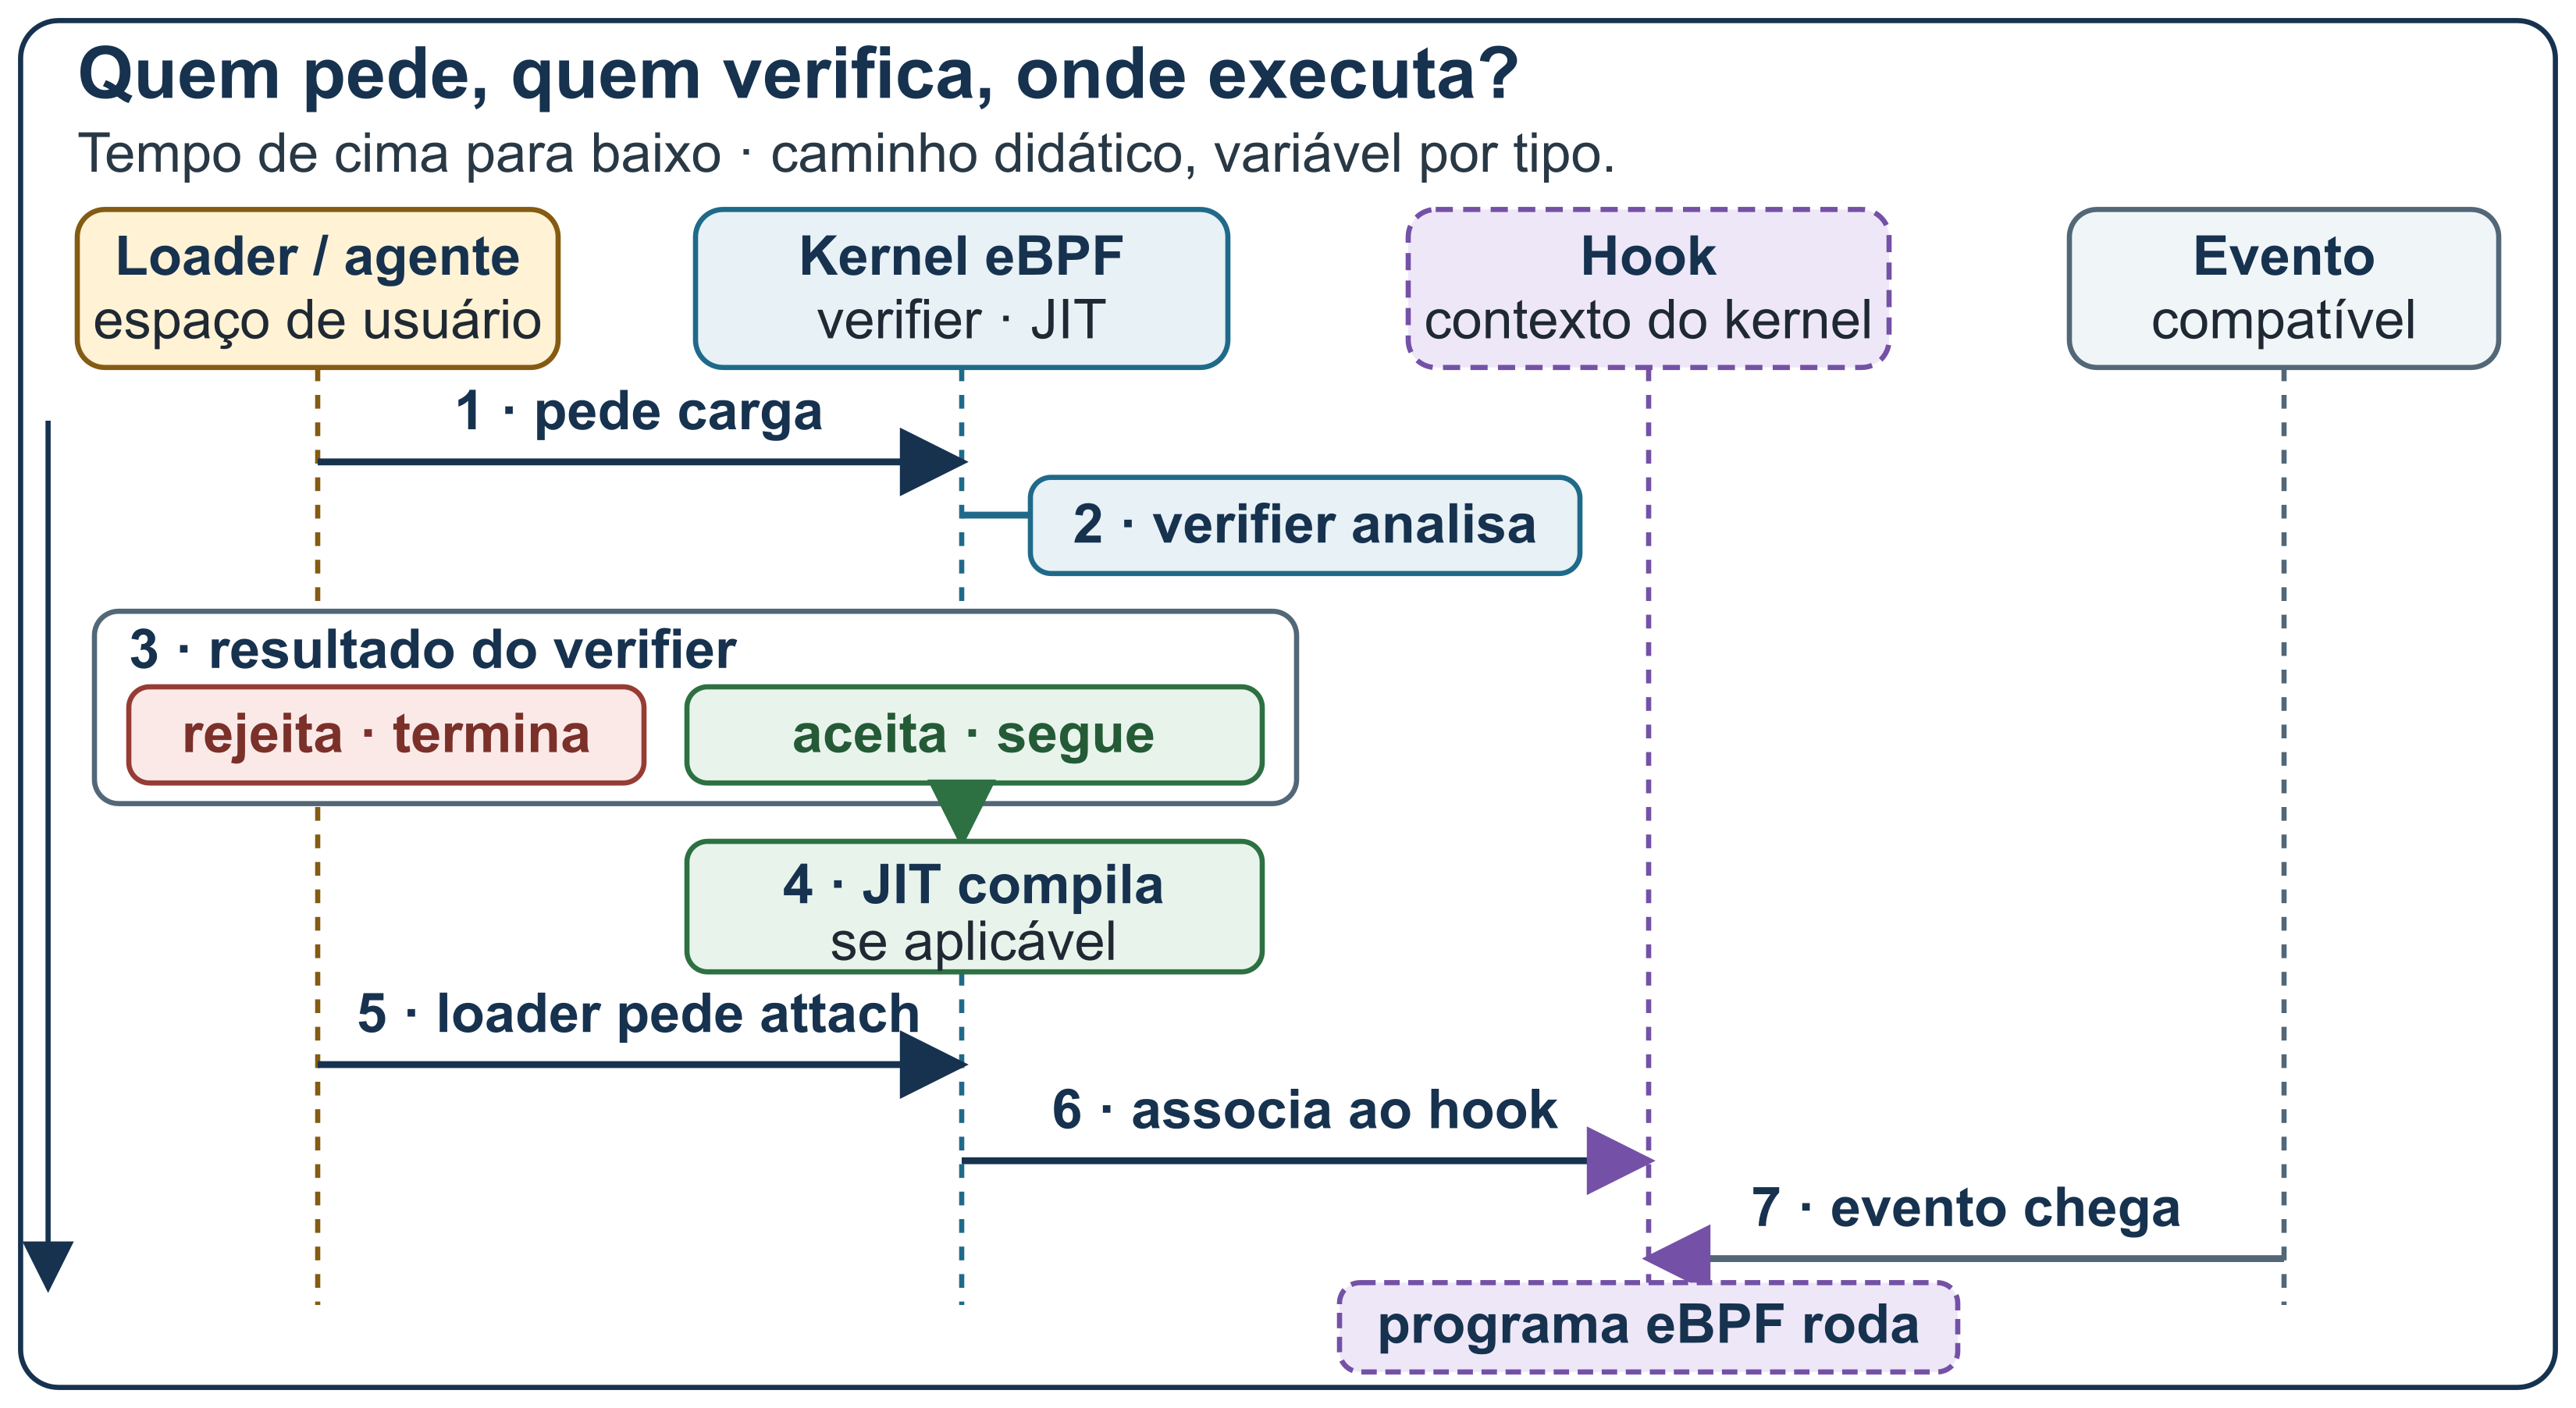
\includegraphics[width=\textwidth,height=0.72\textheight,keepaspectratio]{diagramas/ebpf-cilium-iniciantes/figura-02-sequencia.png}
\fonte{Elaboração própria (2026), com base em (eBPF Foundation, 2026) e (Linux
Kernel Documentation, 2026).}
\end{figure}

\section{Aceito ou rejeitado: o alcance do verifier}\label{aceito-ou-rejeitado-o-alcance-do-verifier}

O verifier analisa tipos, estado, acessos à memória e caminhos. Se não prova as condições aplicáveis, rejeita a carga. Se aceita, o programa passou nessas verificações; isso não confirma a intenção lógica. (Linux Kernel Documentation, 2026).

\begin{table}[!htbp]
\caption{Verificações e limites da conclusão}
\footnotesize
\begin{tabularx}{\textwidth}{>{\raggedright\arraybackslash\hsize=0.760\hsize}X>{\raggedright\arraybackslash\hsize=1.178\hsize}X>{\raggedright\arraybackslash\hsize=1.062\hsize}X}
\toprule
\textbf{O verifier analisa} & \textbf{Isso ajuda a estabelecer} & \textbf{Continua sem prova} \\
\midrule
Tipos e estado & uso compatível dos valores acompanhados & que a regra de negócio é a desejada \\
Acessos à memória & respeito aos limites verificados & que um serviço respondeu corretamente \\
Caminhos do programa & que os caminhos analisados atendem às restrições & que o tráfego terá o resultado esperado \\
\bottomrule
\end{tabularx}
\fonte{Elaboração própria (2026), com base em (Linux Kernel Documentation,
2026).}
\end{table}

Leitura do fluxo: se as propriedades não são provadas, a carga é rejeitada; se são, o programa pode seguir para attach, sem validar a lógica desejada.

\begin{figure}[!htbp]
\caption{Decisão do verifier e limite da conclusão}
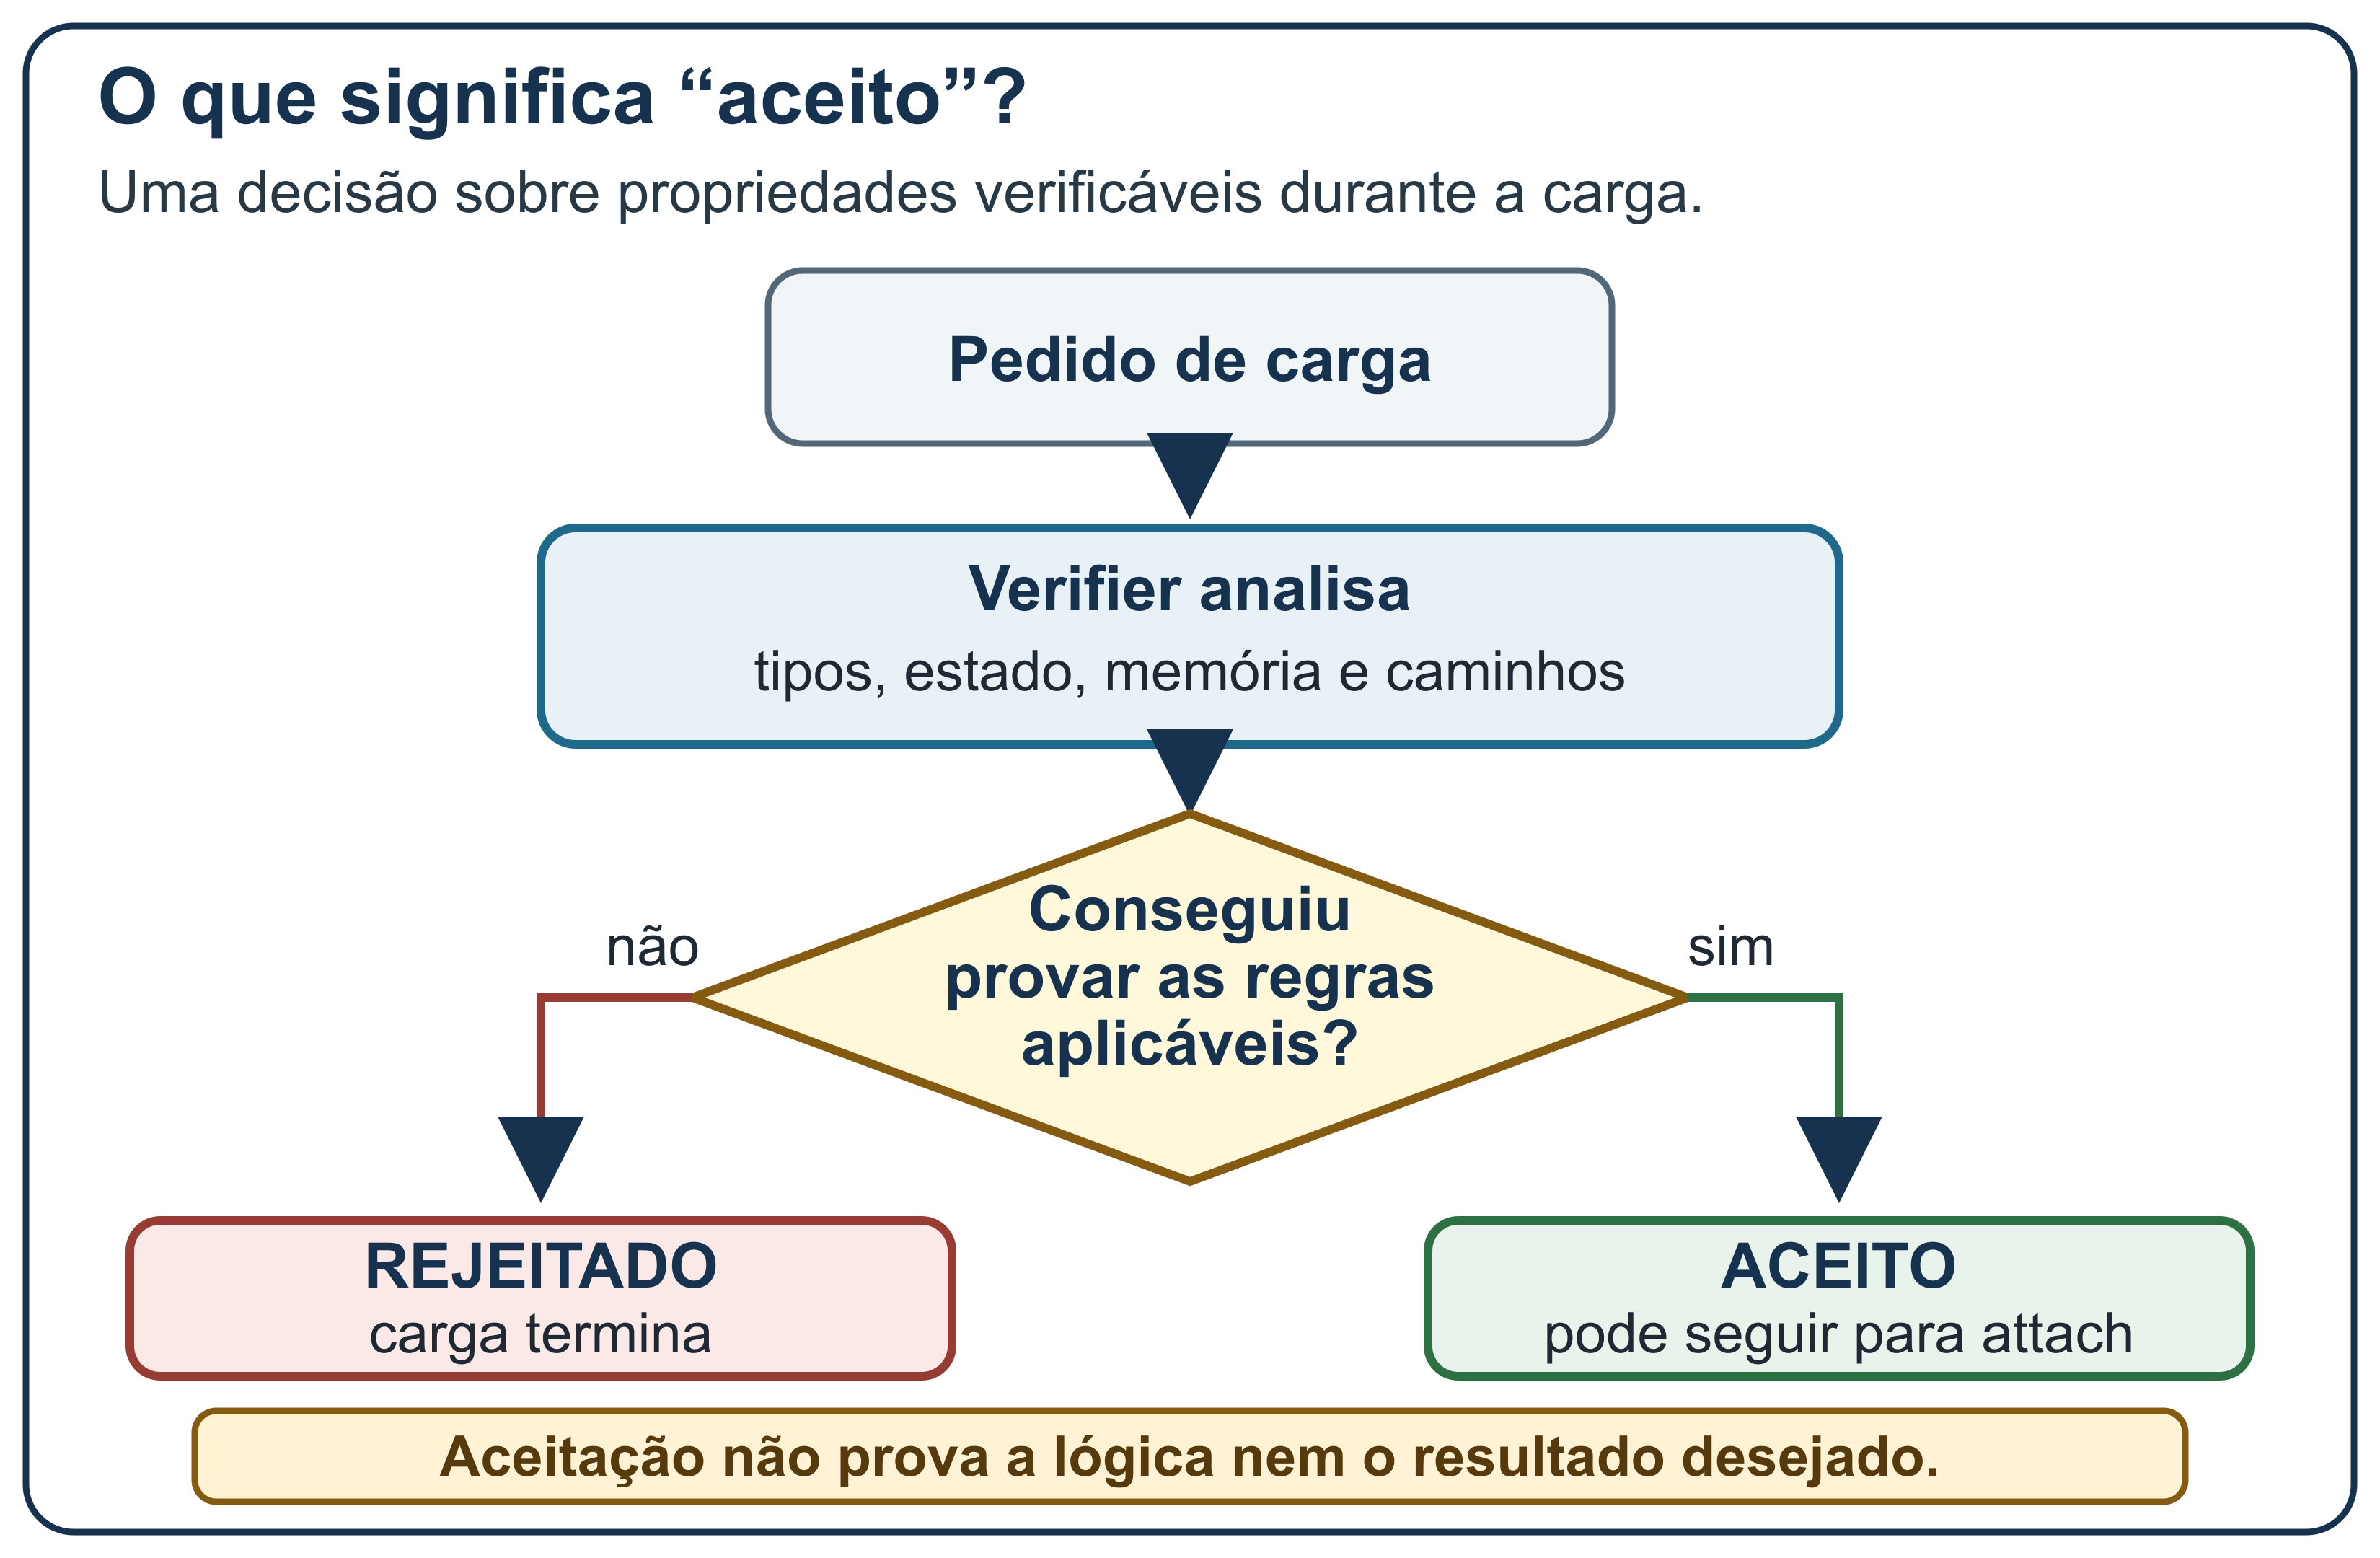
\includegraphics[width=\textwidth,height=0.72\textheight,keepaspectratio]{diagramas/ebpf-cilium-iniciantes/figura-03-decisao.png}
\fonte{Elaboração própria (2026), com base em (Linux Kernel Documentation,
2026).}
\end{figure}

\FloatBarrier

\section{Pratique e confira}\label{pratique-e-confira}

\textbf{Exercício conceitual (15 minutos).} Ordene: (B) solicitar carga, (D) verifier, (F) aceitar/rejeitar, (A) attach, (C) evento e (E) execução. Identifique qual etapa aparece como condicional e em que ponto da sequência ocorre; não execute comandos.

\textbf{Gabarito comentado:} B → D → F; rejeitado, termina. Aceito: a etapa JIT aparece depois da aceitação e antes do attach, quando aplicável; então vêm attach, evento e execução (A → C → E). Isso não prova que a lógica é correta.

\textbf{Perguntas para recordar e transferir:} (1) Hook e evento são iguais? (2) O que o verifier analisa? (3) O que a aceitação não prova? (4) Como diferem agente e datapath?

\textbf{Erro comum:} ``O verifier aceitou, então a policy está correta.'' A conclusão não decorre da verificação: uma análise de segurança de execução não valida, por si só, a intenção lógica ou o comportamento completo da aplicação.

\textbf{Resumo:} o agente configura componentes; o kernel verifica a carga; attach conecta programa e hook; um evento compatível pode executar o programa; aceitar não prova a lógica.

\postextual
\chapter*{Referências}
\addcontentsline{toc}{chapter}{Referências}
\markboth{Referências}{Referências}
\begin{referenciasabnt}

Cilium Authors. Component overview e terminology (documentação stable 1.20.4). {[}s.d.{]}. Acesso em: 28 out. 2026. Disponível em: \href{https://docs.cilium.io/en/stable/overview/component-overview/}{component overview} e \href{https://docs.cilium.io/en/stable/gettingstarted/terminology/}{terminology}.

eBPF Foundation. What is eBPF? {[}s.d.{]}. Acesso em: 28 out. 2026. Disponível em: \href{https://ebpf.io/what-is-ebpf/}{ebpf.io/what-is-ebpf}.

Kubernetes Authors. Labels and selectors. {[}s.d.{]}. Acesso em: 28 out. 2026. Disponível em: \href{https://kubernetes.io/docs/concepts/overview/working-with-objects/labels/}{Kubernetes labels}.

Linux Kernel Documentation. BPF verifier e BPF maps. {[}s.d.{]}. Acesso em: 28 out. 2026. Disponível em: \href{https://docs.kernel.org/bpf/verifier.html}{BPF verifier} e \href{https://docs.kernel.org/bpf/maps.html}{BPF maps}.

\end{referenciasabnt}


\end{document}
